\chapter{Модель специального математического и алгоритмического обеспечения системы анализа, принятия решений и обработки информации в проектировании архитектуры автоматизированных систем управления}\label{ch:ch3}
\section{Основные понятия и определения}\label{sec:ch3/sec1}
Система искусственного интеллекта, которая обрабатывает слабоструктурированную и трудно формализуемую информацию в некоторой предметной области, может интерпретировать и объяснять методы решения задач принятия решения. Экспертные системы способны анализировать и предлагать множество решений на основе некоторых параметрических критериев. Такие системы обрабатывают информацию на основе некоторых формализованных структуированных продукционных правилах логического вывода, в данной работе модулем выявления продукционных правил выступает обработчик нечеткой логики.


Элементами экспертной системы являются следующие модули блоки обработчики:
\begin{enumerate}
    \item база знаний — некоторое семантическое представление знаний, формализованных в виде базы фактов,
    \item блок логического выводе — блок, который моделирует механизм продукционных правил на основе правил логического вывода,
    \item блок интерпретаций — блок, который интерпретирует некоторое семантическое представление получаемых системой данных,
    \item блок формирования рекомендаций — данный блок формирует рекомендации.
\end{enumerate}
Таким образом система поддержки принятия решения, основанные на экспертных систмах главным образом опираются на модуль формирования продукционных правил.

\section{Требования к модели поддержки принятия решений}\label{sec:ch3/sec2}
Требования для разработки системы поддержки принятия решений вырабатываются на основе анализа проблем в области задачи принятия решений. Например, для поддержки принятия решений в области проектирования программного обеспечения крайне сложно аализировать организацию шаблонов проектрования кода на уровне отношений между сущности, также довольно сложнореализуемой задачей является анализ индексации таблиц и определения внешний и составных ключей, отношений между таблицами в БД.
Таким образом, основными требованиями при разработке модели поддержки принятия решений выступили требования по формированию вектора рекомендаций для проектирования того или иного набора инструментов для реализации задач проектирования. Для решения такой задач, после проведения анализа проблематики и выявления альтернатив, была разработана модель нйеронной сети на основе нечеткой логики. Требования к модели принятия решений блоком нейронной сети, главным образом, определялся возможностью реализации продукционного вывода на основе базы знаний, но с возможностью обновления и адаптации под пользовательские запросы. Система должна уметь адаптироваться под запросы пользователей, а также адаптировать свою семантическую продукционную структуру дополняя базу новыми фактами, новыми прецендентами.
Основные требования при проектирования модели поддержки принятия решений перечислены здесь:
\begin{enumerate}
	\item система должна уметь интерпретировать слабоструктурированный текст в семантически верное продукционное правило,
	\item система должна уметь выявлять эвристические закономерности и аппроксимировать функционал оптимизации подбора рекомендаций,
	\item система должна уметь выявлять продукцоинные правила,
	\item система должна уметь обрабатывать отношения между объектами,
	\item система должна уметь формировать рекомендацию.
\end{enumerate}


\subsection{Модель информационного обмена при проектировании системы поддержки прнятия решения}\label{sec:ch3/sec2/sub1}
На рисунке ~\cref{fig:NNmodel} представлена работа блоков обработчиков нейронной сети. Все блоки взаимосвязаннеы друг с другом и образуют интеллектуальную модель поддержки принятия решений.
\begin{figure}[ht]
    \centerfloat{
        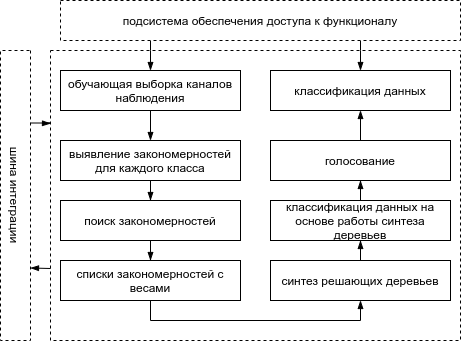
\includegraphics[scale=0.8]{Dissertation/images/DISSER-1.png}
    }
    \caption{Модель нейронной сети}\label{fig:NNmodel}
\end{figure}

Основные блоки интеллектуального модуля поддержки принятия решений это:
\begin{enumerate}
\item база объектов, описывающая параметры конфигурации типовых информационных систем,
\item база знаний прецендентов, сформированная базой объектов,
\item продукционная нечеткая база знаний, формируемая на основе фактов и правил продукционного формирования правил, получаемых из базы знаний,
\item нейронечеткий механизм, который обучается и формирует  нечеткую функцию рекомендаций,
\item блок адаптации данных, данный блок принимает на вход данные получаемые от пользовательских запросов к системе,
\item блок обучения нейронной сети, где происходит обучение нейросетевого механизма,
\item механизм поиска по прецендентам, где происходит обработка запросов и сопостовление процедента с предъявляемым параметром.
\end{enumerate}

На рисунке ~\cref{fig:NNproc} представлена модель обработки данных нейросетевой моделью в укрупненном масштабе. 
\begin{figure}[ht]
    \centerfloat{
        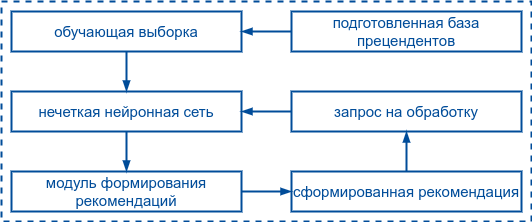
\includegraphics[scale=0.8]{Dissertation/images/DISSER-2.png}
    }
    \caption{Модель нейронной сети}\label{fig:NNproc}
\end{figure}

Если рассматривать задачу с точки зрения теории управления, то мы получаем адаптивную комбинированную систему автоматизированного управления (т.к. обучение происходит с участием человека) с возмущением. 
Управляющая система представлена на рисунке ~\cref{fig:NNsau} в укрупненной абстракции. 
\begin{figure}[ht]
    \centerfloat{
        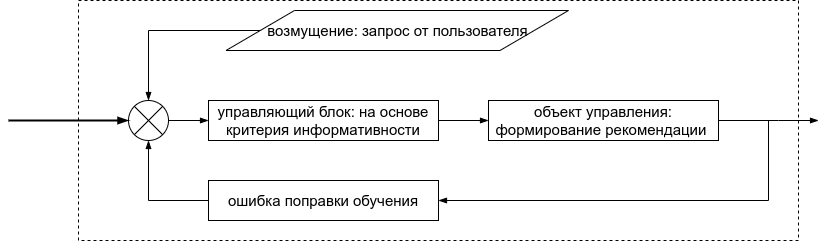
\includegraphics[scale=0.5]{Dissertation/images/DISSER-3.png}
    }
    \caption{Модель нейронной сети}\label{fig:NNsau}
\end{figure}

Сравнительная таблица методов управления представлена на Рисунке ~\cref{fig:Csau}
\begin{figure}[ht]
    \centerfloat{
        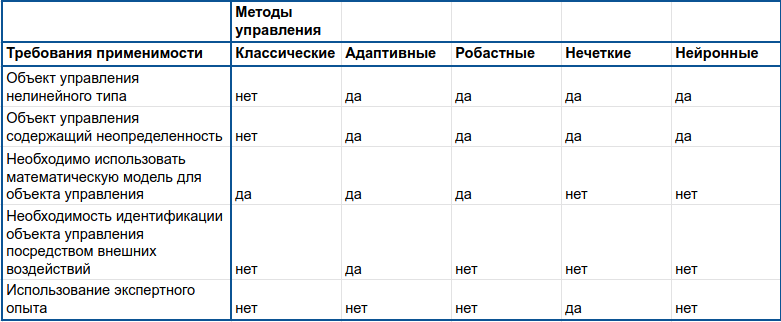
\includegraphics[scale=0.65]{Dissertation/images/DISSER-19.png}
    }
    \caption{Сравнительная таблица методов управления}\label{fig:Csau}
\end{figure}

Модель поддержки принятия решения может быть рассмотрена, как система автоматического управления с возмущением комбинированного типа. Входная информация поступает на линейный вход в модель обаботки информации и структуризации семантических данных ${z}$, обратная связь послупает от модуля расчета ошибки работы нейронной сети, здесь к управляющей системе возвращается информация о состоянии объекта управления ${у}$. Информация о состоянии объекта управления и возмущении ${w}$ поступает на вход к объекту управления, далее информация обрабатывается в соответствии с целью формирования рекомендаций, где объект управления получает воздействия от блока управления в виде набора рекомендаций и в виде управляющих воздействий передается на объект управления
\begin{equation}
    \label{eq:equation30}
    S = \{S_y, O_y, C,  \overrightarrow{z}, \overrightarrow{y}, \overrightarrow{w}\}
\end{equation}

Модель вычислений представлена в виде
\begin{equation}
    \label{eq:equation30}
    E_S=<K_B,F_B,R_B,I^e,R^e>
\end{equation}


где $K_B$- база знаний в виде продукционных правил; 

$F_B$- таблица фактов $S$;

$R_B$- таблица продукционных выводов, создаваемая модулем интерпретатором в ходе вычислений, содержит информацию о причинах возникающих изменений в базе правил, а также поправки, комментарии, внесенные экспертом в базу знаний для объяснений; 

$R^e$ — отношения между объектами; 

$I^e$ — интерпретатор, который опирается на последовательное исполнение: $I^e =<I^{e1}, I^{e2}, I^{e3}, I^{e4}>$,

$I^{e1}$ - процесс выбора из базы знаний подмножества необходимых продукицонных правил; 

$I^{e2}$ - процесс сверки с прецендентами; 

$I^{e3}$ - процесс принятия оптимального решения; 

$I^{e4}$ — процесс исполнения правила.

Модель системы интеллектуального вывода может быть представлена следующим образом
\begin{equation}
    \label{eq:equation31}
    NN=<A_r,X,Y,M^n,E_d,I^{n1}, I^{n2} >,
\end{equation}

где $A_r$ — топология нейронной сети; 

$X, У$ - множества входов и выходов нейронной сети соответственно; 

$М^n$ — множество искусственных нейронов; 

$E_d$ — обучающая и тестирующая выборки; 

$I^{n1}, I^{n2}$ — интерпретаторы обучения и вычислений нейронной сети.

Таким образом, интегрированная нейронная сети для экспертного вывода модели вычислений будет иметь следующий вид
\begin{equation}
    \label{eq:equation32}
    NES=<K_B,X,Y,M^n,E_d,R_e, I^{n1}, I^{n2} >
\end{equation}

В экспертной системе с нейронной сетью сохраняется база правил экспертной системы, с помощью которой строится нейронная сети с некоторыми входами $X$ и выходами $Y$, где $E_d$ — обучающая и тестирующая выорки нейронной сети;  $I^{n1}, I^{n2}$ — интерпретаторы проектируемые для обучения нейронной сети, а также для формирования рекомендаций соответственно; новая система получает новый набор отношений между объектами в виде $R_e$.

Разработанная в работе модель экспертной системы с нейронной сетью проектируется с целью формировать реккомендации. Для извлечений рекомендаций необходимо ввести данные о проектируемой системе согласно шаблону опроса, затем запустить модуль принятия решений. 
Модель вычислений с использованием методов продукционной логики на основе прецедентов имеет следующий вид
\begin{equation}
    \label{eq:equation33}
    PS=<K_{B1},K_{B2},A(p), I^p >
\end{equation}

где $K_{B1},K_{B2}$- блок прецедентов и блок знаний о проектированнии архитектуры; 

$А(р)$ — алгоритм, который определяет схожие прецеденты р.

Интерпретатор $І_р$, использующий алгоритм $А(р)$ и модуль $К_{В2}$, который обрабатывает данные, хранящиеся в базе знаний $К_{B2}$. Все это может быть представлена как совокупность процессов
\begin{equation}
    \label{eq:equation34}
    I^p = <I^{p1}, I^{p2}, I^{p3}, I^{p4}>
\end{equation}

где $I^{p1}$ - сохранение, 

$I^{p2}$ - обнаружение, 
$I^{p3}$ - адаптация , 
$I^{p4}$ - пересмотр

Гибкость модели обучения записит от следущих параметров

\begin{equation}
    \label{eq:equation35}
    NES^p=<K_B,X,Y,M^n,E_d,R_n, I^{np}, I^{n2}, I^p >
\end{equation}

Продукционные правила сохраняются в виде $K_{B1}$, также в виде прецедентов $K_{B2}$ ; $R^n$ — отношения между объектами представляются в виде некоторого отношения вложенности или принадлежности (определяется семантическим интерпретатором логики). Поиск решений разбивается на решение полуаемое с помощью аппроксимации нечеткой логики и работы по выявления прецендентов на основе работы нейронной сети $І^р$ с действием алгоритма $А(р)$ определения похожих прецедентов. Обучение $І^р$ производится на основе данных из прецедентов, также на основе дополнений новыми знаниями от авторизованных пользователей экспертов.


\subsection{Модель принятия решений в модуле поддержки принятия решений}\label{sec:ch3/sec2/sub2}

Представим модель в виде некоторой нелинейной системы:
\begin{equation}
    \label{eq:equation36}
    \[ \varphi(y(x)) = \left\{\begin{array}{ll} x_i, i   = 0,1, ...,  n,\textrm{,}\\ y_k = f_y(x_1,x_2,...,x_n), k = 1,2,...,q & \end{array} \right. \]
\end{equation}

Представим множество возможных значений в следующем виде:
\begin{equation}
    \label{eq:equation37}
    U = \{u_j, u_{j+1},.., u_m\}
\end{equation}

где $u_j$ - оценка, которая проставляется в соответсвии с входной информацией в систему,

$m$ - мощность множества.

Решением задачи будет составление такого множества значений $Y*= \{y_1^*, y_2^*, ..., y_n^*\}$ на постившее множество $X* = \{x_1^*, x_2^*,...,x_n^*\}$. Таким образом, на множество, поступающих значений $X*$ формируется множство выходных значений $Y*$.
Для установления зависимости между объектами выразим эвристическую закономерность в виде обработки семантических лингвистических переменных. Для этого выразим объекты через некоторые терм множества:
\begin{equation}
    \label{eq:equation38}
    A = \{a_j, a_{j+1}, ..., a_m\}
\end{equation}
Данные семантические терм определяются на основе соотношения
\begin{equation}
    \label{eq:equation38}
    a_j = \sum_{p=1}^l\frac{\mu^{a_{j}(u^p_j)}}{u^p_j}
\end{equation}

$\mu^{a_{j}(u^p_j)}$ - степень принадлежности,

$u^p_j$ - объект принадлежности.

Степень принадлежности определяется на основе рангов принадлежности и определяется на основе соотношений следующей системы:
\begin{equation}
    \label{eq:equation40}
    \[ R(\mu) = \left\{\begin{array}{ll} \frac{\mu_1}{\r_1} = \frac{\mu_2}{\r_2} = ... = \frac{\mu_m}{\r_m}, i   = 0,1, ...,  m,\textrm{,}\\ \sum_{i=1}^m{\mu_i} = 1  & \end{array} \right. \]
\end{equation}
В соответствии с нормировкой находим:
\begin{equation}
    \label{eq:equation41}
    \[ R(\mu) = 
    \left\{\begin{array}{ll} 
    \mu_{n-1} = (1 + \frac{r_n}{r_{n-1}} + \frac{r_{n+1}}{r_{n-1}} + ... )^{-1} \textrm{,} 
    \\ \mu_{n+m} = (\frac{r_{n-1}}{r_n} + \frac{r_{n+1}}{r_n} + ... )^{-1}  & \end{array} \right. \]
\end{equation}

Получаемая матрица обладает следующими свойствами:
\begin{enumerate}
    \item транзитивность,
    \item симметричность,
    \item диагональность.
\end{enumerate}

На основании этих свойств выведем соотношение:
\begin{equation}
    \label{eq:equation42}
    s_{ij} = \frac{s_{kj}}{s_{ki}}
\end{equation}

На основе матрицы парных рангов составляется соотношение со значениями 9-ти бальной шкалы Саати 
На рисунке ~\cref{fig:ST} представлена 9-ти бальная шкала Саати.
\begin{figure}[ht]
    \centerfloat{
        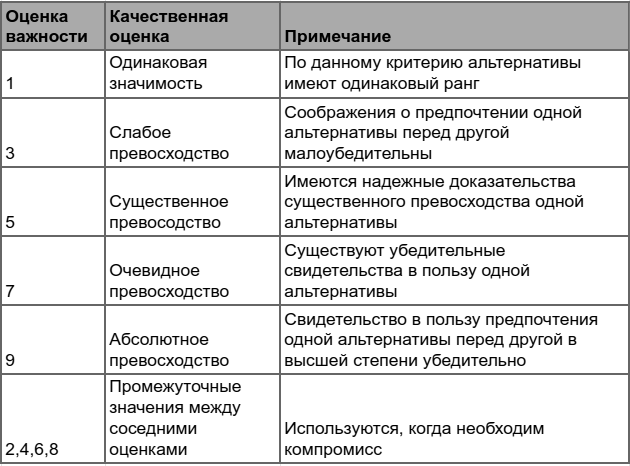
\includegraphics[scale=0.59]{Dissertation/images/APP-1.png}
    }
    \caption{9-ти бальная шкала Саати}\label{fig:ST}
\end{figure}

Приведем перечень функций принадлежности классов. Функция принадлежности к некоторому классу $s$ приведена в ~\cref{eq:equation43}.
\begin{equation}
    \label{eq:equation43}
    s(x,a,b,c) = \left\{\begin{array}{ll} 
    0, x\leq{a} \textrm{,} 
    \\ 2{\frac{x-a}{c-a}}^2, a\leq x\leq b    \\
    1 - 2{\frac{x-c}{c-a}}^2, b\leq x\leq c   \\ 
    1, x\geq c & \end{array} \right. \]
\end{equation}

где $b = \frac{a+c}{2}$.

Продукционное правило интерпретируется на основе:
\begin{equation}
    \label{eq:equation44}
    (i): Q ; P; A \rightarrow B;S,F,N
\end{equation}

где $(i)$ - имя нечеткого правила,

$Q$ - домен нечеткого правила,

$P$ - условия принятия, критерий принятия,

$A \ rightarrow B$ = ядро нечеткого продукционного правила,

$B$ - результирующее заключение, следствие,

$\rightarrow$ - знак продукционной секвенции,

$S$ - метод определения количественной истинности,

$F$ - коэффициент истины,

$N$ - ограничения продукционного вывода.


База знаний в соответствии с представление в виде продукционных правил образует совокупность множество, представимое в некоторой совокупности таблиц фактов.
Термы множества задаются с стандартной форме в виде логических отношений. База знаний задается в виде набора полей, объединенных некоторым логическим отношением, записанных в некоторой таблице совокупности фактов, на основании которых выводится продукционное правило.
Нечеткая база знаний может быть представлена в следующей виде в виде функции Мамдани

\begin{equation}
    \label{eq:equation45}
    \bigcup_{p=1}^{t_k} [\bigcap_{i=1}^{n} \(x_i = a_j^{kp}\)]   \rightarrow  \bigcup_{p=1}^{t_k} [ \bigcap_{k=1}^{q} \(y_k = b_j^{kp}\)  ]
\end{equation}

где  $j = {1,2, ..., q}$, $k = {1,2, ..., q}$, $p = {1,2, ..., t_k}$

База знаний формируется в соответствии с Рисунком ~\cref{fig:KBase}. Структура матрицы знаний представлена с Рисунком ~\cref{fig:ST}.
\begin{figure}[ht]
    \centerfloat{
        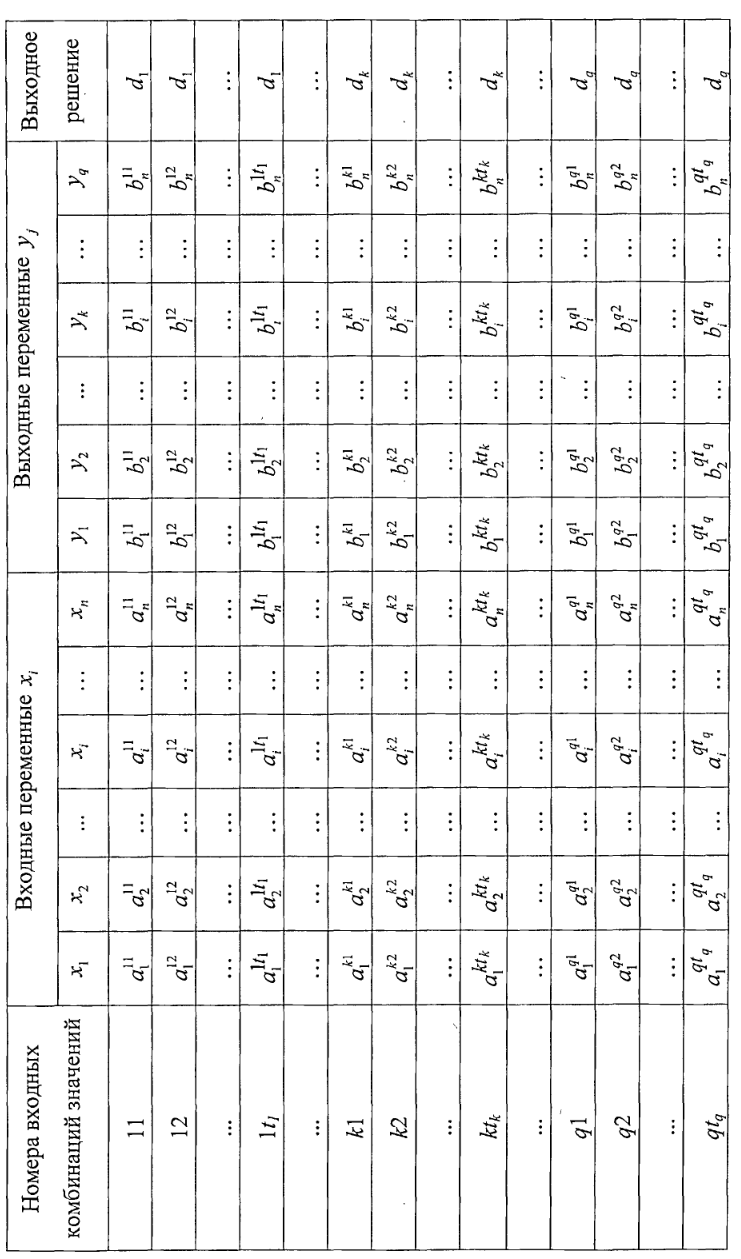
\includegraphics[scale=0.5]{Dissertation/images/DISSER-7.png}
    }
    \caption{Структура матрицы знаний}\label{fig:KBase}
\end{figure}


\subsection{Алгоритм оценки устойчивости специального математического и алгоритмического обеспечения проектирования архитектуры}\label{sec:ch3/sec2/sub3}
Рассмотрим следующую систему. Пусть система поддержки решений будет представлена в виде:
\begin{equation}
    \label{eq:equation46}
     \left\{\begin{array}{ll} 
    \dot{x} = X(x,t) \textrm{,} 
    \\ X(0,t) = 0 \textrm{,} 
     \forall{t} \geq t_0
      & \end{array} \right. \]
\end{equation}


Пусть отклик от обучения будет представлен в виде постоянного возмущения $R(x,t)$
\begin{equation}
    \label{eq:equation47}
    \dot{x} = X(x,t) + R(x,t)
\end{equation}

где $R(0,t) \neq 0$ и момент покоя $x = 0$ не является решением данного уравнения.

Положение системы, согласно \cite{Tau}, будет определено, как устойчивое при постоянно действующих возмущениях, если будет существовать такое малое $\varepsilon$ для которого найдутся такая пара положительных $\delta_0$ и $\delta_1$, что при выполнении неравенства $|R(x,t)| < \delta_1$ при всех $|x|\leq \varepsilon$ и $t \geq t_0$, движение возмущения может быть описано неравенством $|x(x^0, t)| < \varepsilon$ и $t \geq t_0$.
В общем смысле система поддержки решений на основе модуля нейронной сети при малых отклонениях обучения на нейронную сеть малы т.е. отклонение положения возмущения от невозмущенного положения малы. Определим меру возмущений, согласно теореме Малкина \cite{Tau}
\begin{equation}
    \label{eq:equation48}
    |grad V(x,t)| = \sqrt{\sum_{i=1}^n{\frac{\partial V}{\partial x_i}}^2} \leq N
\end{equation}

где $N$ - положительная константа.

Тогда, система принятий решений и интеллектуальный модуль должны быть ограничены в отклонениях в возмущениях в виде некоторой константы $N$. Таким образом, переобучение или недобучение системы определяются, как состояния, которые выходят за предел допустимого $N$ отклонений в возмущениях.

Выведем последовательность действий при обработке информации в модулей нейронной сети на основе нечеткого модуля продукционных правил. Представим перечень шагов:
\begin{enumerate}
    \item ввод данных в систему, система получает набор переменных, которые принимают конкретные значения в зависимости от значений введенных данных, данные передаются на вход, множество введенных данных обозначим как $P =\{p_1, p_2, ..., p_n\}$,
    \item сохраняем набор параметров в сущность, создаем сущность описание прецендента,
    \item определяем важности параметров, присваиваем весовые коэффициенты каждому параметру $W = \{W_1, W_2, ..., W_n\}$
    \item сохраняем размерность количества признаков, введеных в систему,
    \item переводим значения характеристик в числовые переменные посредством фукционалов принадлежности,
    \item передаем на обработку в нейронную сеть для поиска по таблице фактов,
    \item создаем сущность для агрегированная и обработка промежуточной информации, 
    \item проходим в цикле по всем продукционным правилам и сохраняем найденное в агрегированную сущность,
    \item в случае отсутствия данных создаем отдельную подсущность для хранения пустых множеств значений параметров переменных отображения, жанная подсущность будет помогать основному каналу наблюдения аппроксимировать данные черех обработку обратного обучения черех нейронные связи,
    \item в сущносте с отобранными по рангам соответствия всем значениям, проверяем на метрическую приналдежность векторов признаков к вектору введенных переменных, используется евклидова метрика $D(P,A_j) = \sqrt{\sum_{i=1}^n{a_i - p_i}^2w_i}$, где прецедент, находящийся в обработке $A_j$ сравнивается с описанным вектором пересенных запросом $P$, сравнения проходят согласно векторам важности в упорядоченном множестве,
    \item производим расчет евклидовой метрики расстояния $D$, 
    \item рассчитываем расстояния для граничных объектов $D_{max}(P) = \sqrt{\sum_{i=1}^n{p_{max} - p_{min}}^2w_i}$,
    \item расчитываем шаги сходства, степени возможного правдоподобия или близости $S(A,P) = \frac{(1-D)}{D_{max}}$, нормируем и приводим в долевое выражение от $\{0, ..., 1\}$,
    \item в случае, если не находятся похожие прецеденты , передаем запрос на уменьшение уровня правдоподобия и производим расчеты заново,
    \item в случае заполнения значений и отбору прецедентов не по всем переменным, сохраняем то состояние, что есть и выводим ответ,
    \item сформированный ответ сохраняем в продукционную базу прецедентов для последующего использование.
\end{enumerate}

На Рисунке~\cref{fig:NN1} указано исполнения вышеописанных шагов 1-9, на Рисунке~\cref{fig:NN2} все остальные.
\begin{figure}[ht]
    \centerfloat{
        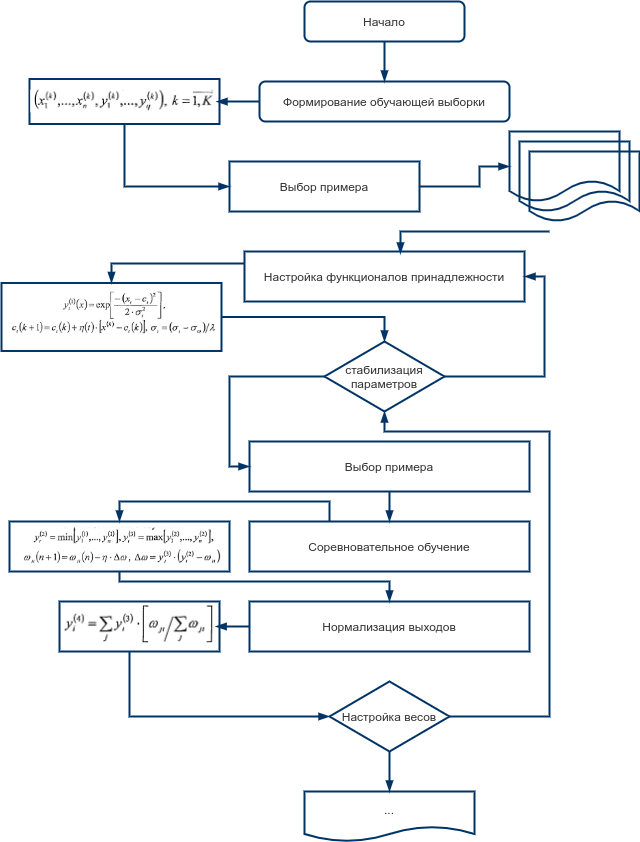
\includegraphics[scale=0.65]{Dissertation/images/DISSER-29.png}
    }
    \caption{Последовательность обработки данных в модуле нейронной сети}\label{fig:NN1}
\end{figure}
\begin{figure}[ht]
    \centerfloat{
        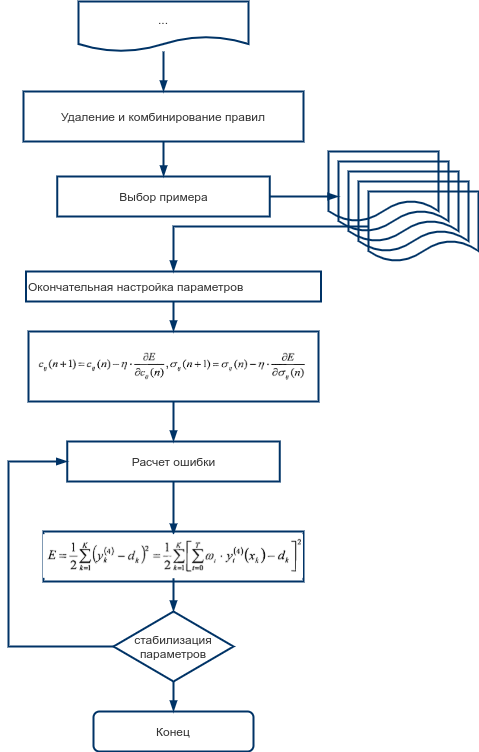
\includegraphics[scale=0.65]{Dissertation/images/DISSER-30.png}
    }
    \caption{Последовательность обработки данных в модуле нейронной сети}\label{fig:NN2}
\end{figure}



\subsection{Математическая модель системы проектирования устойчивой архитектуры программного обеспечения}\label{sec:ch2/sec3/sub1}
Пусть система проектирования представляется в виде положительно определенной функции $V(x,t)$, рассмотрим функцию $\omega_1(x)$, которая выступит ограничением $V(x,t) \geq \omega_1(x)$на функцию работы системы
\begin{equation}
    \label{eq:equation49}
    m = min_{x \in S_{\varepsilon}}\omega_1(x)
\end{equation}

Представим область определения функции $V(x,t)$  в виде некоторой сферы $S_\varepsilon$ при всех $t \geq t_0$
\begin{equation}
    \label{eq:equation50}
    V(x,t) \geq \omega_1(x) \geq m
\end{equation}

Пусть обучение системы выражается как $\dot{V}(x,t)$ в соответствии с представлением ~\cref{eq:equation46} является отрицательной функцией. Тогда, определим положительную функцию $\omega_2(x)$
\begin{equation}
    \label{eq:equation50}
    \dot{V(x,t)} \leq -\omega_2(x) , t \geq t_0
\end{equation}

Таким образом, в силу того, что $\omega_2(x)$ положительно определена существует некоторое $h$, которое удовлетворит условие
\begin{equation}
    \label{eq:equation50}
    \dot{V(x,t)} \leq -\omega_2(x) < -h
\end{equation}

Выразим систему $\dot{V(x,t)}$ согласно ~\cref{eq:equation47} с некоторым возмущением 
\begin{equation}
    \label{eq:equation51}
    \dot{V(x,t)} = \frac{\partial V}{\partial t} + \sum_{i=1}^n{\frac{\partial V}{\partial x_i}}X_i + \sum_{i=1}^n{\frac{\partial V}{\partial x_i}}R_i = \dot{V} + \sum_{i=1}^n{\frac{\partial V}{\partial x_i}}R_i
\end{equation}

Согласно неравенству Коши-Шварца ~\cite{Korn}
\begin{equation}
    \label{eq:equation52}
    \sum^n_{i=1}{a_ib_i}^2 \leq \sum_{i=1}^n{a^2_i} \sum_{i=1}^n{b^2_i} 
\end{equation}

Получим
\begin{equation}
    \label{eq:equation53}
    |\sum_{i=1}^n{\frac{\partial V}{\partial x_i}}R_i| \leq {\sqrt {\sum_{i=1}^n{\frac{\partial V}{\partial x_i}}}}^2 {\sqrt{\sum_{i=1}^n{R_i}}^2} = |gradV(x,t)||R(x,t)|
\end{equation}

Находим
\begin{equation}
    \label{eq:equation54}
    \dot{V(x,t)} \leq \dot{V(x,t)} +  |\sum_{i=1}^n{\frac{\partial V}{\partial x_i}}R_i| < -h + N |R(x,t)|
\end{equation}

Допустим $|R(x,t)| < \delta_1 = h/(2N), |x| \leq \varepsilon, t \geq t_0$, тогда отклонение возмущения примет вид
\begin{equation}
    \label{eq:equation55}
    \dot{V(x,t)}  < -h/2
\end{equation}

Решение $x(x^0, t)$ при $|x^0|<\delta_0$ удовлетворит условию
\begin{equation}
    \label{eq:equation56}
    |x(x^0,t_0), t_0|  = V(x^0, t_0) < m
\end{equation}

В случае, если отклонение в возмущении будет возрастать и станет больше $m$, то система обучения станет неустойчивой. Для более подробного изучения устойчивости системы нейронной сети с нечеткой логикой можно провести с помощью иных аналитических методов. Такая работа выходит за пределы темы исследования и может быть изучена читателем самостоятельно. Для систематизации методов анализа устойчивости моделей представлен Рисунок~\cref{fig:Trel}.

\begin{figure}[ht]
    \centerfloat{
        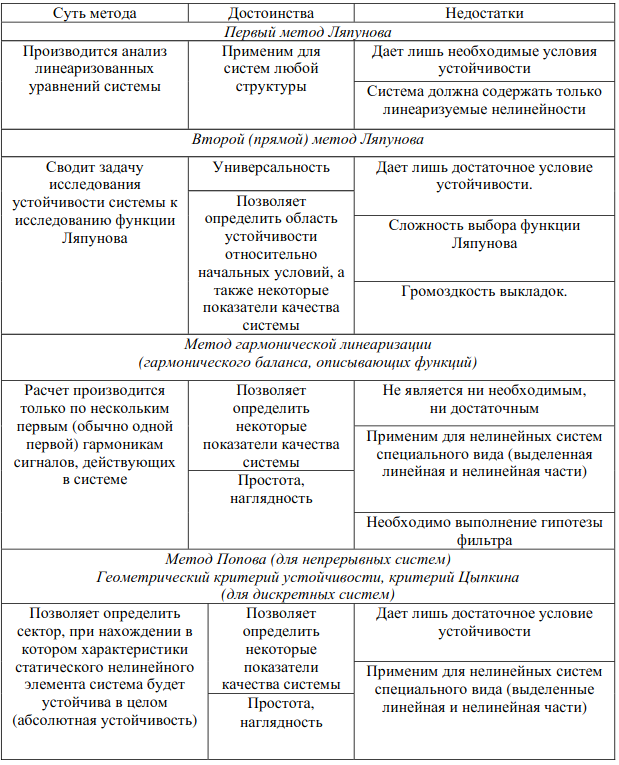
\includegraphics[scale=0.65]{Dissertation/images/DISSER-20.png}
    }
    \caption{Сравнительная таблица применения методов анализа устойчивости}\label{fig:Trel}
\end{figure}

Сравнительная таблица применения методов анализа устойчивости представлена на Рисунке~\cref{fig:Trel}.
\section{Выводы по главе}\label{sec:ch3/conc}
В данной главе решены следующие задачи:
\begin{enumerate}
    \item продемонстрирована математическая модель нейронной сети на основе нечеткого вывода Мамдани. Определены структура отображения входной и выходной информации, процесс обработки, фазификации и дефазификации наборов данных,
    \item разработан алгоритм нейронной сети на основе прецедентов для задач принятия решений,
    \item продемонстрирована природа устойчивости обучения, рассмотренная, как отклонение в возмущениях в нелинейной адаптивной комбинированной системе с возмузением,
    \item продемонстрирована модель продукционного вывода на основе нечетких функционалов принадлежности,
    \item разработана модель формирования базы знаний, на основе таблицы фактов и семантического структурирования лексических термов, проведена работа по моделированию отображения фактов в логические продукционные правила на основе аппроксимации эвристического отображения градиентом.
\end{enumerate}
\clearpage
